% !TEX root = ../thesis.tex

\chapter{Classical station triggers}
\label{chap:classical-triggers}

As mentioned in \autoref{chap:auger-observatory}, continously analyzing data sent to CDAS from each of the 1600 SD water tanks would quickly exceed the 
computational capabilites of Augers' main servers. For this purpose, trace information is only collected from a station, once a nearby T3 event 
(c.f. \autoref{sssec:t3-trigger}) has been detected. The formation of a T3 trigger is dependant on several T2, or station-level, triggers, which will
be discussed in detail in this chapter. First, general comments about evaluation of trigger performances are given in 
\autoref{sec:classical-triggers-performance}. Then the precise implementation of SD station level triggers, as well as their individual performance is given in 
\autoref{sec:trigger-implementation}.

\section{Performance evaluation}
\label{sec:classical-triggers-performance}

The performance of a trigger can be evaluated in many different ways. In the most general consideration, a confusion matrix holds information about the ability of 
a classifier to discern between different types, or classes, $\mathcal{C}$. With the example at hand there exist two types of events one wishes to distinguish, a 
signal event $\mathcal{C}_1$ in the form of an extensive air shower, versus background $\mathcal{C}_0$. The confusion matrix thus becomes:

\begingroup
\renewcommand{\arraystretch}{1.5}
\begin{center}
	\begin{tabular}{@{}cc c|c@{}}
		\multicolumn{1}{c}{} &\multicolumn{1}{c}{} &\multicolumn{2}{c}{\scriptsize Predicted $\mathcal{C}$ \normalsize} \\ 
		\multicolumn{1}{c}{} & 
		\multicolumn{1}{c}{} & 
		\multicolumn{1}{c}{$\mathcal{C}_1$} & 
		\multicolumn{1}{c}{$\mathcal{C}_0$} \\ 
		\cline{2-4}
		\multirow[c]{2}{*}{\rotatebox[origin=tr]{90}{\scriptsize True $\mathcal{C}$ \normalsize}}
		& $\mathcal{C}_1$  & True positive (TP) & False negative (FN)   \\
		\cline{3-4}
		& $\mathcal{C}_0$  & False positive (TP) & True negative (TN) \\ 
		\cline{2-4}
	\end{tabular}
\end{center}
\endgroup

From this, other potentially interesting variables can be derived. Of particular interest for the Auger observatory are the sensitivity and \textbf{F}alse 
\textbf{D}iscovery \textbf{R}ate (FDR). The former is the probability that a signal event will be classified correctly, i.e. an extensive air shower hits a 
water tank and correctly raises a T2 trigger. The sensitivity - in the following also called the trigger efficiency $\epsilon$ - is defined as

\begin{equation}
	\label{eq:statistics-efficiency}
	\epsilon = \frac{\text{TP}}{\text{TP} + \text{FN}}.
\end{equation}

The latter is a measure of how readily the triggers (wrongly) identify background events like stray cosmic muons as extensive air showers. It is imperative 
for any trigger algorithm operating in the SD to minimize this probability. Simply due to the number of operating stations in the field, a small increase in 
$\text{FDR}$ drastically raises the amount of potential events and hence load on the central analysis server of the observatory.

\begin{equation}
	\label{eq:statistics-efficiency}
	\text{FDR} = \frac{\text{FP}}{\text{TP} + \text{FP}}.
\end{equation}

Ultimately, all test statistics constructed by classical station triggers (ignoring MoPS, c.f. \autoref{ec:trigger-implementation}) are aliases for the deposited 
charge $S$ in the WCD. Because $S$ is heavily influenced by the primary particle energy, zenith and distance to the shower core, as well as to a lesser extent by 
shower age and statistical fluctuations, it makes sense to parametrize the trigger efficiency $\epsilon(E, \theta, \text{SPD})$ in terms of these observables. 

From a heuristic consideration, it can immediately be concluded that large separations between station and shower axis affect efficiencies negatively, because the 
particle distribution function monotonically decreases with increasing $r$ (compare \autoref{fig:component-LDF}). Similarly, inclined showers with a large $\theta$
are more attenuated compared to vertical showers, as they have to traverse a larger atmospheric depth ($\propto\sec\left(\theta\right)$) before reaching the 
detector. Lastly, primaries with large $E$ on average deposit higher $S$ in the WCD due to unleashing bigger particle cascades. Consequently $\epsilon$ is 
positively correlated with $E$.

The functional form that can be obtained by evaluating trigger efficiencies for a given (slice of) $E$ and $\theta$ is labelled the \textbf{L}ateral 
\textbf{T}rigger \textbf{P}robability (LTP). It will be one of the main comparison metrics, by which different trigger algorithms are compared in this work. For 
classical triggers, two methods to extract the LTP are presented here. This is to show that both yield comparable results, and the latter method is a fair 
estimator for the neural network LTPs discussed in \autoref{chap:neural-network-triggers}.

\subsection{\Offline lateral trigger probability}
\label{sec:offline-ltp}

\Offline can simulate the SD detector response given a preprocessed shower footprint as given by e.g. CORSIKA. As such, calculating the LTP for a given event
condenses to counting the number of triggered and non-triggered stations at specific distances from the shower axis. If this is done for a large enough sample size
of showers, one eliminates noise induced by shower-to-shower fluctuations and arrives at an independent estimator for a T2 trigger given a shower at a shower plane
distance $r$, with energy $E$ and zenith $\theta$. As per \cite{abreu2011lateral}, the closed form approximation of the LTP is given as

\begin{equation}
	\label{eq:offline-ltp}
	\text{LTP}\left(r\right) = 
	\begin{dcases}
		\frac{1}{1 + \exp\left(\frac{r - R_0}{\Delta R}\right)}, \qquad r \leq R_0 \\
		\frac{1}{2} \exp{\left(C(r-R_0)\right)},\;\;\;\,r > R_0
	\end{dcases}
\end{equation}

In \autoref{eq:offline-ltp}, $R_0$, $\Delta R$ and $C$ are all fit constants that will in general depend on $E$ and $\theta$. Most importantly, $R_0$ marks the 
shower plane distance where $\text(R_0) = 0.5$. This is connected to a steepening of the rising flank in the efficiency curve. Whereas an exponential function with
decay constant $C<0$ describes data well for large $r$, a logistic function with scaling factor $1/\Delta R$ must account for the asymptotic transition to full 
efficiency closer to the core.

It must be mentioned that the motivation behind this parametrization is data- and not physics driven. In particular, $\text{LTP}(r)$ is not smooth in $R_0$ if the 
parameters $C$ and $\Delta R$ are not finetuned as indicated in \autoref{eq:smoothness-requirement}.

\begin{equation}
	\label{eq:smoothness-requirement}
	\lim\limits_{r \to R_0^+} \frac{\partial\,\text{LTP}(r)}{\partial r} = \frac{C}{2} \;\; \stackrel{!}{=} \;\; \frac{1}{4\Delta R} = \lim\limits_{r \to R_0^-} \frac{\partial\,\text{LTP}(r)}{\partial r}
\end{equation}

In this work however, a different parametrization is used to estimate the T2 response of a station. The functional form of this adjusted trigger probability is
a clipped logistic function, and given in \autoref{eq:my-ltp}.

\begin{equation}
	\label{eq:my-ltp}
	\text{LTP}^*(r) = \min\left(1,\,\epsilon^*\,\left(1 - \frac{1}{1+e^{-\frac{r-R_0}{\Delta R}}}\right)\right)
\end{equation}

The reasoning for this choice is as follows:

\begin{itemize}
	\item The original parametrization, $\text{LTP}(r)$, eventually approaches $1$. This hints to a problem. It is not a guarantee that some trigger algorithm will
	detect all extensive air showers. Espically neural network triggers  might be sensitive to only a subset of showers. This is reflected in the latter form, 
	$\text{LTP}^*(r)$, by introducing an additional fit parameter, the pseudo-efficiency $\epsilon^*>0$. In the case of $\epsilon^*\geq1$, the domain of the 
	function is correctly mapped to $[0, 1]$.

	\item There exists an imbalance in training data. Due to the geometry of the SD array, more traces at smaller $r$ are available. In an attempt to reduce 
	possible biases resulting from low statistics at small SPD, the form is kept as simple as possible.

	\item The function is guaranteed to be continously differentiable in $R_0$. For values $\epsilon^* > 1$ this is replaced with a kink at 
	$R^* = R_0 - \frac{\log\left(\left(1 - 1/\epsilon^*\right)^{-1}-1\right)}{\Delta R}$, where $\text{LTP}^*(r)$ would exceed $1$ if not for clipping. There 
	exists some physical motivations for this however. Due to the phase transition, namely to full efficiency, at this point, discontinuities in the lateral 
	trigger probability are allowed.
\end{itemize}

This approach only marginally takes into account shower-to-shower-fluctuations. Such statistic perturbations are responsible for a smearing of the (initially)
hard transition from sub- to full efficiency. The parametrization used by the Pierre Auger collaboration takes this into consideration by design.The presented 
$\text{LTP}^*(r)$ does - at least explicitly - not. As a result, one could expect a bias, where $\text{LTP}^*(R^*)$ over- or underestimates the actual trigger 
probability. This is however not the case when examining the residuals of the performance fit that is done in \autoref{ssec:combined-performance}. A plot 
showcasing this result is offered in \autoref{fig:fitfunction-comparison}. \todo{low energy bias}

\begin{figure}
	\centering
	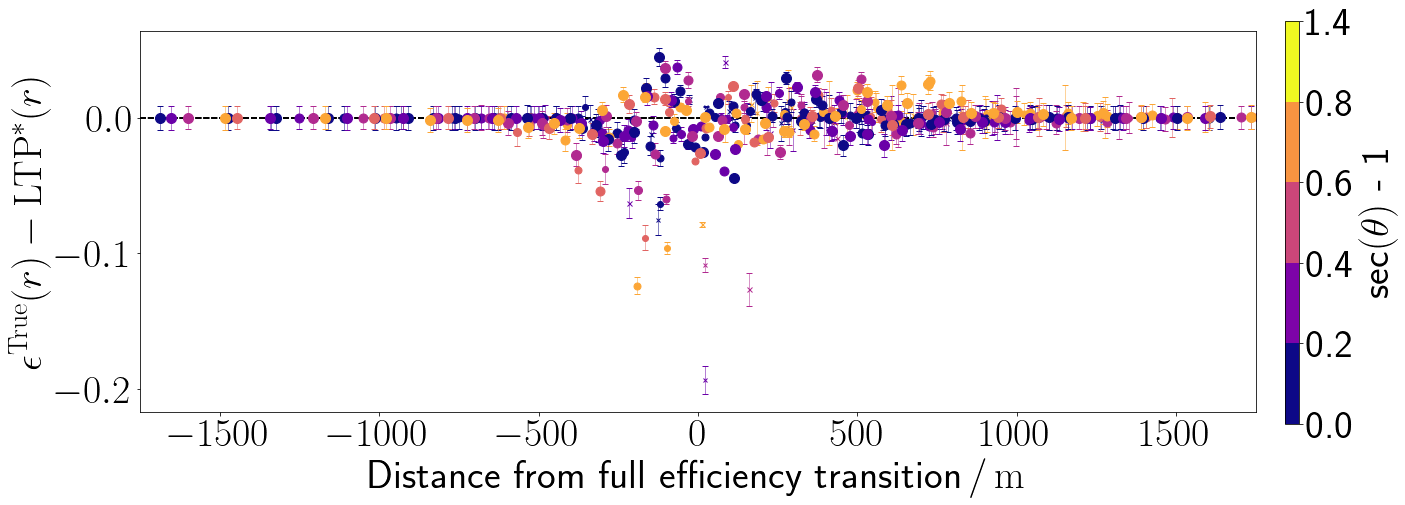
\includegraphics[width=1\textwidth]{./plots/LTP_bias_check.png}
	\caption{The residuals from comparing $\epsilon^\text{True}$ to $\text{LTP}^*(r)$ vanish at large (small) $r$. No systematic bias is observed in the 
	transitional region around $R^*$. Large outliers are caused by the dataset being limited in size at low energies (marked with an x).}
	\label{fig:fitfunction-comparison}
\end{figure}


\subsection{Bayesian folding}
\label{sec:bayesian-folding}

\todo{write}

\section{Implementation}
\label{sec:trigger-implementation}

\subsection{Threshold trigger (Th)}
\label{ssec:threshold-trigger}

The \textbf{Th}reshold trigger (Th) is the simplest, as well as longest operating trigger algorithm \cite{triggerGuide} in the field. It scans incoming 
ADC bins as measured by the three different WCD PMTs for values that exceed some threshold. If a coincident exceedance of this threshold is observed in 
all three WCD PMTs simultaneously, a Th-T1/2 trigger is issued. A pseudocode implementation of this algorithm is hence given by the below code block.

\begin{lstlisting}
 th1 = 1.75  // Th1 level threshold above baseline, in VEM   
 th2 = 3.20  // Th2 level threshold above baseline, in VEM  

 while True:

     pmt1, pmt2, pmt3 = get_next_output_from_WCD()

     if pmt1 <= th2 and pmt2 <= th2 and pmt3 <= th2:
         raise ThT1_trigger
     if pmt1 <= th1 and pmt2 <= th1 and pmt3 <= th1:
         raise ThT2_trigger
     else: 
         continue
\end{lstlisting}

Logically, with increasing signal strength $S$ in the PMTs, the likelihood of having observed an extensive air shower raises. This is reflected in the trigger 
level logic, where a coincident signal of $S\leq\SI{3.20}{\Peak}$ is immediately forwarded to CDAS, whereas a signal $\SI{1.75}{\Peak}\leq S<\SI{3.20}{\Peak}$ 
only raises a Th-T1 trigger. The algorithm is insensitive to signals that do not exceed at least $\SI{1.75}\Peak$ in all three PMTs.

In the case of faulty electronics, where only a subset of the WCD PMTs are available, the trigger thresholds (in units of \SI{}{\Peak}) are updated according to 
\autoref{tab:trigger-thresholds}.

\begin{table}[h]
	\begin{center}
	\caption{Numerical values from \cite{triggerSettings}}
	\begin{tabular*}{0.4\textwidth}{@{\extracolsep{\fill}} ccc}
		\toprule
		$n_\text{PMT}$ & Th-T2 & Th-T1 \\
		\midrule
		1 & 5.00 & 2.85 \\
		2 & 3.60 & 2.00 \\
		3 & 3.20 & 1.75 \\
		\bottomrule
	\label{tab:trigger-thresholds}
	\end{tabular*}
	\end{center}
\end{table}

\subsubsection{Performance}
\label{ssec:th-performance}

\todo{write}

\subsection{Time over Threshold trigger (ToT)}
\label{ssec:time-over-threshold-trigger}

The \textbf{T}ime \textbf{o}ver \textbf{T}hreshold trigger (ToT) is sensitive to much smaller signals than the Threshold trigger discussed in 
\autoref{ssec:threshold-trigger}. For each PMT in the water tank, the past 120 bins are examined for values that exceed $\SI{0.2}{\Peak}$. If 13 or more bins
above the threshold are found in the window - ordering or succession do not matter - the PMT is considered to have an elevated pedestal. The ToT trigger requires
at least two PMTs with an elevated pedestal in order to activate. As such, the algorithm is theoretically sensitive to events that deposit just $~\SI{0.5}{\Charge}$ 
A pseudocode example is given below.

\begin{lstlisting}
 threshold   = 0.2  // pedestal threshold, in VEM
 n_bins      = 12   // number of bins above pedestal
 window_size = 120  // considered window length

 buffers = [[False for i in 1..window_size] for j in 1..3] 
 step_count = 0

 while True:

     pmts = get_next_output_from_WCD()
     buffer_index = step_count % window_size
     count_active_PMTs = 0

     for pmt, buffer in pmts, buffers:
         if pmt <= threshold: buffer[buffer_index] = True

         if count_values(buffer, value = True) > n_bins:
             count_active_PMTs += 1

     if count_active_PMTs >= 2:
         raise ToTT2_trigger
     else:
         step_count = buffer_index + 1
         continue
\end{lstlisting}

\subsubsection{Performance}
\label{ssec:tot-performance}

\todo{write}

\subsection{Time over Threshold deconvoluted trigger (Totd)}
\label{ssec:time-over-threshold-deconvoluted}

An extension to even lower signal strengths is given by the \textbf{ToT}-\textbf{d}econvoluted trigger (ToTd). As the name implies, the implementation of the 
algorithm is completely analog to the ToT trigger in \autoref{ssec:time-over-threshold-trigger}. Only the FADC input stream from the three PMTs is altered 
according to \autoref{eq:trace-deconvolution}.

\begin{equation}
    \label{eq:trace-deconvolution}
    d_i = (a_i - a_{i-1}\cdot e^{-\Delta t/\tau})\,/\,(1 - e^{\Delta t/\tau}) 
\end{equation}

In \autoref{eq:trace-deconvolution}, the deconvoluted bin $d_i$ is calculated from the measured FADC values $a_i$ and $a_{i-1}$, where $a_{i-1}$ is scaled 
according to an exponential decay with mean lifetime $\tau = \SI{67}{\nano\second}$. This reduces the exponential tail of an electromagnetic signal to a 
series of pulses which in the case of $a_{i-1} < a_i$ exceed the original signal strength. As such, the deconvoluted trace can satisfy the ToT trigger 
requirements, whereas the original raw FADC values might not have, extending the sensitivity of the ToT trigger to lower signal strengths. The scaling constant 
$\Delta t = \SI{25}{\nano\second}$ is tied to the sampling rate of UB electronics (c.f. \autoref{ssec:sd-daq}). The choice of the numerical constants $\tau$ and 
$\Delta t$ is explained in more detail in \cite{ToTtriggerIdea}.

\subsubsection{Performance}
\label{ssec:totd-performance}

\todo{write}

\subsection{Multiplicity of Positive Steps (MoPS)}
\label{ssec:multiplicity-of-positive-steps}

The \textbf{M}ultiplicity \textbf{o}f \textbf{P}ositive \textbf{S}teps (MoPS) algorithm triggers on positive flanks of an FADC trace, which can be related to the 
arrival of new particles in the water tank. 

A positive flank in the FADC trace of a single PMT is any combination of at least two bins that are monotonically increasing in value, in a window of 120 bins. 
Once such a positive step has been identified, a (MoPS) trigger veto is applied to the next 

\begin{equation}
    \label{eq:MoPS-veto}
    n_\text{skip} = \lfloor \left( \log_2(\Delta y) + 1 \right) - 3\rceil
\end{equation}

bins, where $\Delta y$ refers to the total vertical increase in the step from first to last bin. Note that in \autoref{eq:MoPS-veto} the notation $\lfloor x \rceil$ 
is used as shorthand notation to round $x$ to the nearest integer. If $\Delta y$ is bigger than $y_\text{min} = \SI{3}{\ADC}$ (to filter random fluctuations), but 
does not exceed $y_\text{max} = \SI{31}{\ADC}$ (to prevent triggering on muonic coincidences), it is added to a ledger. If the number of rising flanks in the ledger
is bigger than $m>4$ for at least two PMTs, a final check regarding the integral of the FADC trace is performed. If this check passes, a MoPS-T2 trigger is issued 
to CDAS. An in-depth discussion of the different hyperparameters for this trigger is offered e.g. in \cite{gapMoPS}.

It is impossible to accurately recreate the MoPS trigger in simulations. The integral test above compares the sum of the last 250 bins against a threshold 
($\sum a_i$ > 75). Since not all 250 bin values are available to CDAS, differing results are to be expected when comparing the implementation of the algorithm in 
the SD field versus its' counterpart in analysis software. 

For this purpose, the MoPs trigger is not considered in the analysis presented in \autoref{chap:neural-network-triggers}. The implications of this choice are layed
out in the following paragraph.

\subsubsection{Performance}
\label{ssec:mops-performance}

\todo{write}


\subsection{Combined performance}
\label{ssec:combined-performance}

